\section{人工智能与应用}\index{人工智能与应用}

\begin{enumerate}
%% ============= 1
\item 答案:A。选项B:教材举过一个例子:符号无法表达“仓禀实而知礼节”所蕴含的丰富内涵。选项C:问题引导下的人工智能学习方法是“行为主义”,这是一种通过问题引导,尝试解决问题,根据结果反馈来调整学习方法的强化学习。“依赖知识库,通过推理来解决问题”是符号主义。选项C:1956年美国达特茅斯学院召开的人工智能研讨会标志这人工智能学科的正式诞生,而符号主义、联结主义、行为主义是逐步形成的流派。

%% ============= 2
\item 答案:B。

%% ============= 3
\item 答案:D。人工智能研究的至少是某种程序设计语言下程序代码的编写。伪代码是一种程序设计语言、自然语言、数学符号相互夹杂的不可执行的算法表示方法,不是人工智能研究领域。

%% ============= 4
\item 答案:C。要重视书本的例子:机器人客服与人工客服协同完成服务是混合增强人工智能,混合增强人工智能实例还有:通过用户手机搜索记录和位置移动数据来感知人群移动,预测景点拥堵情况;人机协同太公机器人;军事协同作战机器人;达芬奇外科手术机器人。

%% ============= 5
\item 答案:C。考查人工智能对社会的影响
	\begin{enumerate}[label=\Alph*.]
	\item 人工智能成本只会越来越低,一些领域的工人会被自动化所取代。
	\item 人工智能既能监控全局数据,又能完成数据分析和资源调配。
	\item 这是“机器人三守则”的第2守则。
	\item 人工智能并不是单一的技术,它能融入现有生产中,国内已有很多企业向“智能化”转型了。
	\end{enumerate}

%% ============= 6
\item 答案:B。可以从信息系统的“输入、存储、处理、输出”四个功能和过程去考虑,当然这里没有表述到“存储”。由此,步骤①的输出是最后的。步骤③的输入是第一步的——可惜四个选项都这样的顺序。不过②④⑤的顺序还是容易区分的:先定位(②),再分割(④),最后识别(⑥),答案选B。

%% ============= 7
\item 答案:B。
	\begin{enumerate}[label=$(\arabic*)$]
\setcounter{qnumber}{1}
\begin{lstlisting}[numbers=left]
import matplotlib.pyplot as plt
import pandas as pd
# 创建画布和坐标系, 此处代码略
df = pd.read_excel("data.xlsx")  # 读取点的坐标值并完成分类存储
x = df["宽度"]
y = df["高度"]
t = df["类别"]
x1 = []; y1 = []; x2 = []; y2 = []
for i in range(`\clozeblank{2}`):
    if t[i] == "柠檬":
        x1.append(x[i]);  y1.append(y[i])
    else:
        `\clozeblank{2}`
# 绘制散点图
plt.scatter(x1, y1, c="r", marker="*", s=15, label="柠檬")
plt.scatter(x2, y2, c="b", marker="o", s=5, label="苹果")
# 显示图例、设置坐标轴后最后显示散点图。此处代码略
\end{lstlisting}
	\item 从第$5 \sim 7$行程序看,$x,y,t$三个变量分别保存了原始数据的每一列(Series),从第10行的t[i]使用方式上看,$i$就是索引号,因此第①空的范围与数据行数有关,答案是\lstinline|len(t)|。第11行程序将柠檬的宽高保存到了$x1,y1$中,那么else分支应该保存苹果的数据,答案是\lstinline|x2.append(x[i]);  y2.append(y[i])|。程序第15、16行绘制了两个散点图,后面几个参数的功能可以了解一下:参数c是color的别名,可以绘制散点的色彩,r就是red,b就是blue;参数marker是散点的样式,“*”表示五角星形,“o”表示稍大的圆点;参数s是size的别名,意味散点的大小;label就是当调用plt.legend()函数时显示的图例中的标签。
\begin{lstlisting}[numbers=left]
kk = [0, 0.1, 0.2, 0.3, 0.4, 0.5, 0.6, 0.7, 0.8, 0.9, 1, 1.1, 1.2, 1.3, 1.4, 1.5, 1.6, 1.7, 1.8, 1.9, 2.0, 3.0, 4.0]
bb = [0, 0.5, 1, 1.5, 2, 2.5, 3, 3.5, 4, 4.5, 5, 5.5, 6, 6.5, 7, 7.5, 8, 8.5, 9, 9.5, 10]

def loss(k, b):    
    n = 0						# 变量n存储总的错误个数
    for i in range(len(x1)):    # 统计柠檬分类的错误个数        
        if y1[i] < k * x1[i] + b:
            n += 1
    `\clozeblank{2}`  		# 统计苹果分类的错误个数
    return n
minloss = 30
for k in kk:
    for b in bb:
        minloss1 = loss(k, b)
        if minloss1 < minloss:
            minloss = minloss1
            K = k
            B = b
print("求得分类直线的k=", K, "b=", B)
# 绘制直线,此处代码略
\end{lstlisting}
\begin{figure}[h!]
\centering
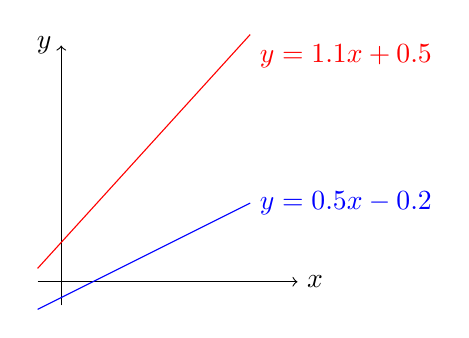
\begin{tikzpicture}[domain=-.3:2.4]
%\draw[thick,color=gray] (-0.1,-1.1) grid (3.9,3.9);
\draw[->] (-.3,0) -- (3,0) node[right] {$x$};
\draw[->] (0,-.3) -- (0,3) node[left] {$y$};
\draw[color=blue] plot (\x, {0.5*(\x) - 0.2}) node[right] {$y=0.5x - 0.2$};
\draw[color=red] plot (\x, {1.1*(\x) + 0.5}) node[below right] {$y=1.1x+0.5$};
\end{tikzpicture}
\end{figure}


	\item 这题有点数学的味道。对于数学函数$y = kx + b$,对于不同的$k,b$组合,产生的函数图像是不一样的,如上图所示。因此主程序第12、13行用两重循环枚举了不同$k,b$的组合,对于每一组$k,b$组合都使用函数loss()计算出位柠檬和苹果分类错误的个数,通过打擂法保留分类错误最小时的$k,b$组合。由此分析,第③空处的代码于第6行的循环类似——第6行的循环遍历了列表$x1, y1$中柠檬的宽度和高度值,对于柠檬而言,$y$值应该大于$kx+b$的值,因此它用条件\lstinline|y1[i] < k * x1[i] + b|来统计错误的数量。苹果可以模仿着写:数据在列表$x2, y2$中,苹果正常的$y$值应该小于$kx+b$,因此程序可以写成:
\begin{lstlisting}[frame=none]
for i in range(len(x2)):
    if y2[i] > k * x2[i] + b:
        n += 1
\end{lstlisting}
	\item 可以有两种方法判定:①将水果宽度$x=6.8$代入$y=0.4x+5$,得$y=7.72$,即分类器计算得到苹果和柠檬的高度分界点是7.72厘米,现在水果的高度是7.3厘米,小于临界点,应该为苹果。②将高度值$y=7.3$代入$y=0.4x+5$,得$x=5.75$,即宽度分界点是5.75厘米,而该水果得宽度是6.8厘米,大于分界点,应该判定为苹果。
	\end{enumerate}









\end{enumerate}


\newpage
